% Created by tikzDevice version 0.9 on 2016-04-28 16:54:50
% !TEX encoding = UTF-8 Unicode
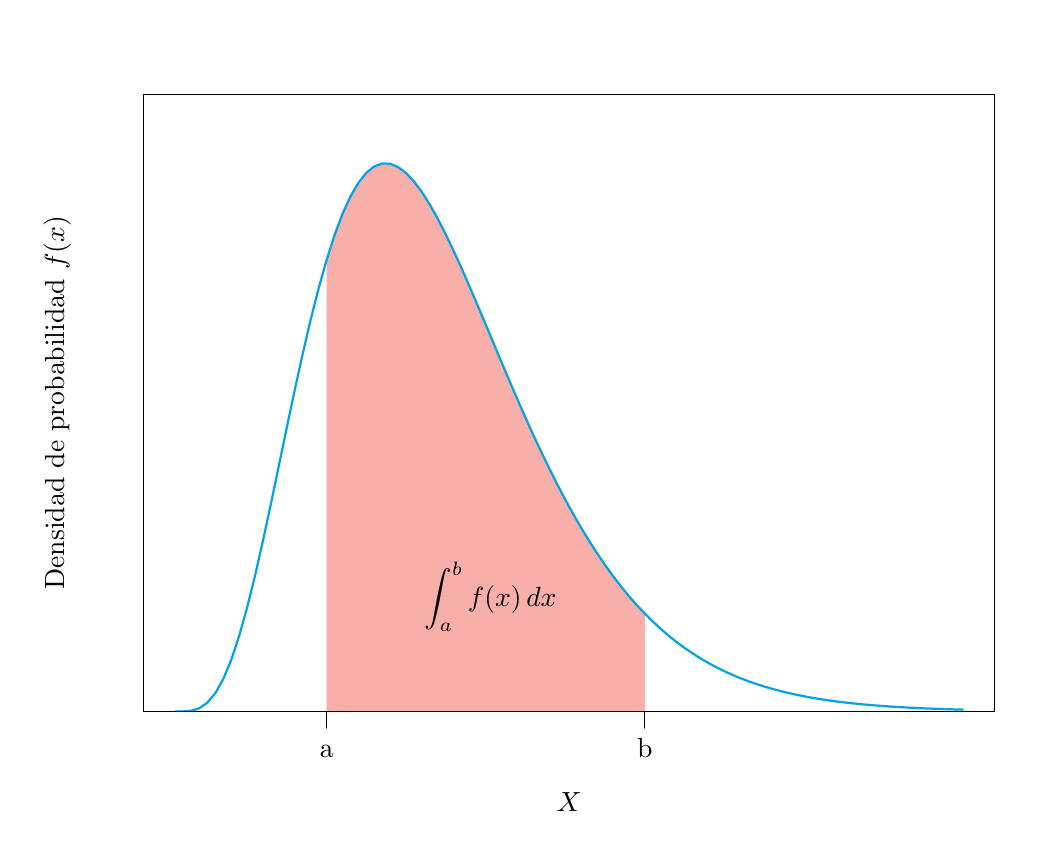
\begin{tikzpicture}[x=1pt,y=1pt]
\definecolor{fillColor}{RGB}{255,255,255}
\path[use as bounding box,fill=fillColor,fill opacity=0.00] (0,0) rectangle (361.35,289.08);
\begin{scope}
\path[clip] (  0.00,  0.00) rectangle (361.35,289.08);
\definecolor{drawColor}{RGB}{0,0,0}

\node[text=drawColor,anchor=base,inner sep=0pt, outer sep=0pt, scale=  1.00] at (195.67,  6.00) {$X$};

\node[text=drawColor,rotate= 90.00,anchor=base,inner sep=0pt, outer sep=0pt, scale=  1.00] at ( 13.20,153.54) {Densidad de probabilidad $f(x)$};
\end{scope}
\begin{scope}
\path[clip] (  0.00,  0.00) rectangle (361.35,289.08);
\definecolor{drawColor}{RGB}{0,0,0}

\path[draw=drawColor,line width= 0.4pt,line join=round,line cap=round] (108.00, 42.00) -- (222.98, 42.00);

\path[draw=drawColor,line width= 0.4pt,line join=round,line cap=round] (108.00, 42.00) -- (108.00, 36.00);

\path[draw=drawColor,line width= 0.4pt,line join=round,line cap=round] (222.98, 42.00) -- (222.98, 36.00);

\node[text=drawColor,anchor=base,inner sep=0pt, outer sep=0pt, scale=  1.00] at (108.00, 25.20) {a};

\node[text=drawColor,anchor=base,inner sep=0pt, outer sep=0pt, scale=  1.00] at (222.98, 25.20) {b};
\end{scope}
\begin{scope}
\path[clip] ( 42.00, 42.00) rectangle (349.35,265.08);
\definecolor{fillColor}{RGB}{238,50,36}

\path[fill=fillColor,fill opacity=0.39] (108.00, 42.00) --
	(108.00,205.09) --
	(110.87,214.08) --
	(113.75,221.76) --
	(116.62,228.08) --
	(119.50,233.03) --
	(122.37,236.65) --
	(125.25,238.95) --
	(128.12,240.01) --
	(131.00,239.90) --
	(133.87,238.71) --
	(136.75,236.53) --
	(139.62,233.46) --
	(142.50,229.60) --
	(145.37,225.05) --
	(148.24,219.92) --
	(151.12,214.30) --
	(153.99,208.28) --
	(156.87,201.95) --
	(159.74,195.38) --
	(162.62,188.66) --
	(165.49,181.84) --
	(168.37,174.99) --
	(171.24,168.15) --
	(174.12,161.39) --
	(176.99,154.73) --
	(179.86,148.21) --
	(182.74,141.86) --
	(185.61,135.71) --
	(188.49,129.77) --
	(191.36,124.06) --
	(194.24,118.58) --
	(197.11,113.35) --
	(199.99,108.38) --
	(202.86,103.65) --
	(205.74, 99.18) --
	(208.61, 94.96) --
	(211.49, 90.98) --
	(214.36, 87.24) --
	(217.23, 83.73) --
	(220.11, 80.44) --
	(222.98, 77.38) --
	(222.98, 42.00) --
	cycle;
\definecolor{drawColor}{RGB}{5,161,230}

\path[draw=drawColor,line width= 0.8pt,line join=round,line cap=round] ( 53.38, 42.00) --
	( 56.26, 42.02) --
	( 59.13, 42.26) --
	( 62.01, 43.14) --
	( 64.88, 45.11) --
	( 67.76, 48.52) --
	( 70.63, 53.63) --
	( 73.51, 60.51) --
	( 76.38, 69.14) --
	( 79.25, 79.36) --
	( 82.13, 90.94) --
	( 85.00,103.57) --
	( 87.88,116.95) --
	( 90.75,130.71) --
	( 93.63,144.55) --
	( 96.50,158.14) --
	( 99.38,171.21) --
	(102.25,183.52) --
	(105.13,194.86) --
	(108.00,205.09) --
	(110.87,214.08) --
	(113.75,221.76) --
	(116.62,228.08) --
	(119.50,233.03) --
	(122.37,236.65) --
	(125.25,238.95) --
	(128.12,240.01) --
	(131.00,239.90) --
	(133.87,238.71) --
	(136.75,236.53) --
	(139.62,233.46) --
	(142.50,229.60) --
	(145.37,225.05) --
	(148.24,219.92) --
	(151.12,214.30) --
	(153.99,208.28) --
	(156.87,201.95) --
	(159.74,195.38) --
	(162.62,188.66) --
	(165.49,181.84) --
	(168.37,174.99) --
	(171.24,168.15) --
	(174.12,161.39) --
	(176.99,154.73) --
	(179.86,148.21) --
	(182.74,141.86) --
	(185.61,135.71) --
	(188.49,129.77) --
	(191.36,124.06) --
	(194.24,118.58) --
	(197.11,113.35) --
	(199.99,108.38) --
	(202.86,103.65) --
	(205.74, 99.18) --
	(208.61, 94.96) --
	(211.49, 90.98) --
	(214.36, 87.24) --
	(217.23, 83.73) --
	(220.11, 80.44) --
	(222.98, 77.38) --
	(225.86, 74.52) --
	(228.73, 71.86) --
	(231.61, 69.38) --
	(234.48, 67.09) --
	(237.36, 64.96) --
	(240.23, 63.00) --
	(243.11, 61.18) --
	(245.98, 59.51) --
	(248.85, 57.96) --
	(251.73, 56.54) --
	(254.60, 55.24) --
	(257.48, 54.04) --
	(260.35, 52.95) --
	(263.23, 51.94) --
	(266.10, 51.02) --
	(268.98, 50.18) --
	(271.85, 49.41) --
	(274.73, 48.71) --
	(277.60, 48.07) --
	(280.48, 47.49) --
	(283.35, 46.96) --
	(286.22, 46.48) --
	(289.10, 46.05) --
	(291.97, 45.65) --
	(294.85, 45.29) --
	(297.72, 44.97) --
	(300.60, 44.67) --
	(303.47, 44.40) --
	(306.35, 44.16) --
	(309.22, 43.94) --
	(312.10, 43.75) --
	(314.97, 43.57) --
	(317.84, 43.41) --
	(320.72, 43.26) --
	(323.59, 43.13) --
	(326.47, 43.02) --
	(329.34, 42.91) --
	(332.22, 42.82) --
	(335.09, 42.73) --
	(337.97, 42.65);
\definecolor{drawColor}{RGB}{0,0,0}

\node[text=drawColor,anchor=base,inner sep=0pt, outer sep=0pt, scale=  1.00] at (167.22, 80.06) {$\displaystyle \int_a^b f(x)\,dx$};
\end{scope}
\begin{scope}
\path[clip] (  0.00,  0.00) rectangle (361.35,289.08);
\definecolor{drawColor}{RGB}{0,0,0}

\path[draw=drawColor,line width= 0.4pt,line join=round,line cap=round] ( 42.00, 42.00) --
	(349.35, 42.00) --
	(349.35,265.08) --
	( 42.00,265.08) --
	( 42.00, 42.00);
\end{scope}
\end{tikzpicture}
